\chapter{Testing Methodology and Results}
\section{Test Matrices}
The project is geared towards matrices which occur in circuit simulations and hence
such matrices are the ain focus of the test set. These matrices are taken from the 
SuiteSparse Matrix Collection (formerly known as the University of Florida Sparse Matrix Collection).
These matrices are stored in Matlab structure files.

\section{Performance Testing}
The scheduler generates a cycle accurate schedule hence is sufficient to 
extract performance related information. Hence the performance can be done
without running the tests on the hardware. This type of testing allows us to 
gain insights about the most contributing factors without worrying about the 
synthesizability of the hardware configuration. We have simulated a range
of hardware configuration and the performance variations are mentioned in the following 
subsections.

\subsection{Variation with Number of Processing Elements}
The number of cycles required for factorization should reduce with the number of
processing elements because more number of nodes can be assigned simultaneously.
For large matrices this may be true but for the smaller matrices, like the ones used
in the test, there is no enough parallelism and the performance saturates after 4
processing elements. Hence for the hardware synthesizable design we can set number of
processing elements to be 4.

\begin{table}[H]
    \centering
    \caption{Hardware configuration for testing variation with number of PES}
    \label{tab:res:peVar:hwConfig}
    \begin{tabular}{L{6cm} L{1.5cm}}
        \toprule
        Parameter & Value \\
        \midrule
        Number of PEs           & Variable  \\
        Number of BRAMs         & 16         \\
        Number of Ports/ BRAM   & 4         \\
        Read Latency of BRAM    & 2          \\
        Latency of MAC Unit     & 20          \\
        Latency of Divider Unit & 31          \\
        \bottomrule
    \end{tabular}
\end{table}

\begin{table}[H]
    \centering
    \caption{Performance variation with the number of PES}
    \label{tab:res:peVar:data}
    \begin{tabular}{l l l l l l l} 
        \toprule
        Matrix Name & Order  & NNZ & 2 PEs & 4 PEs & 8 PEs & 16 PEs \\
        \midrule
        $fpga\_dcop\_01$ & 1813 & 5892 &         2923   &     2149    &    2154  &      2150   \\
        $fpga\_dcop\_04$ & 1220 & 5884 &         3021   &     2255    &    2252  &      2252   \\
        $fpga\_dcop\_50$ & 1220 & 5892 &         3303   &     2433    &    2435  &      2431   \\
        $rajat11$      & 135    &  665 &          856   &      848    &     848  &       848    \\
        \bottomrule
    \end{tabular}
\end{table}



\begin{figure}[H]
    \centering
    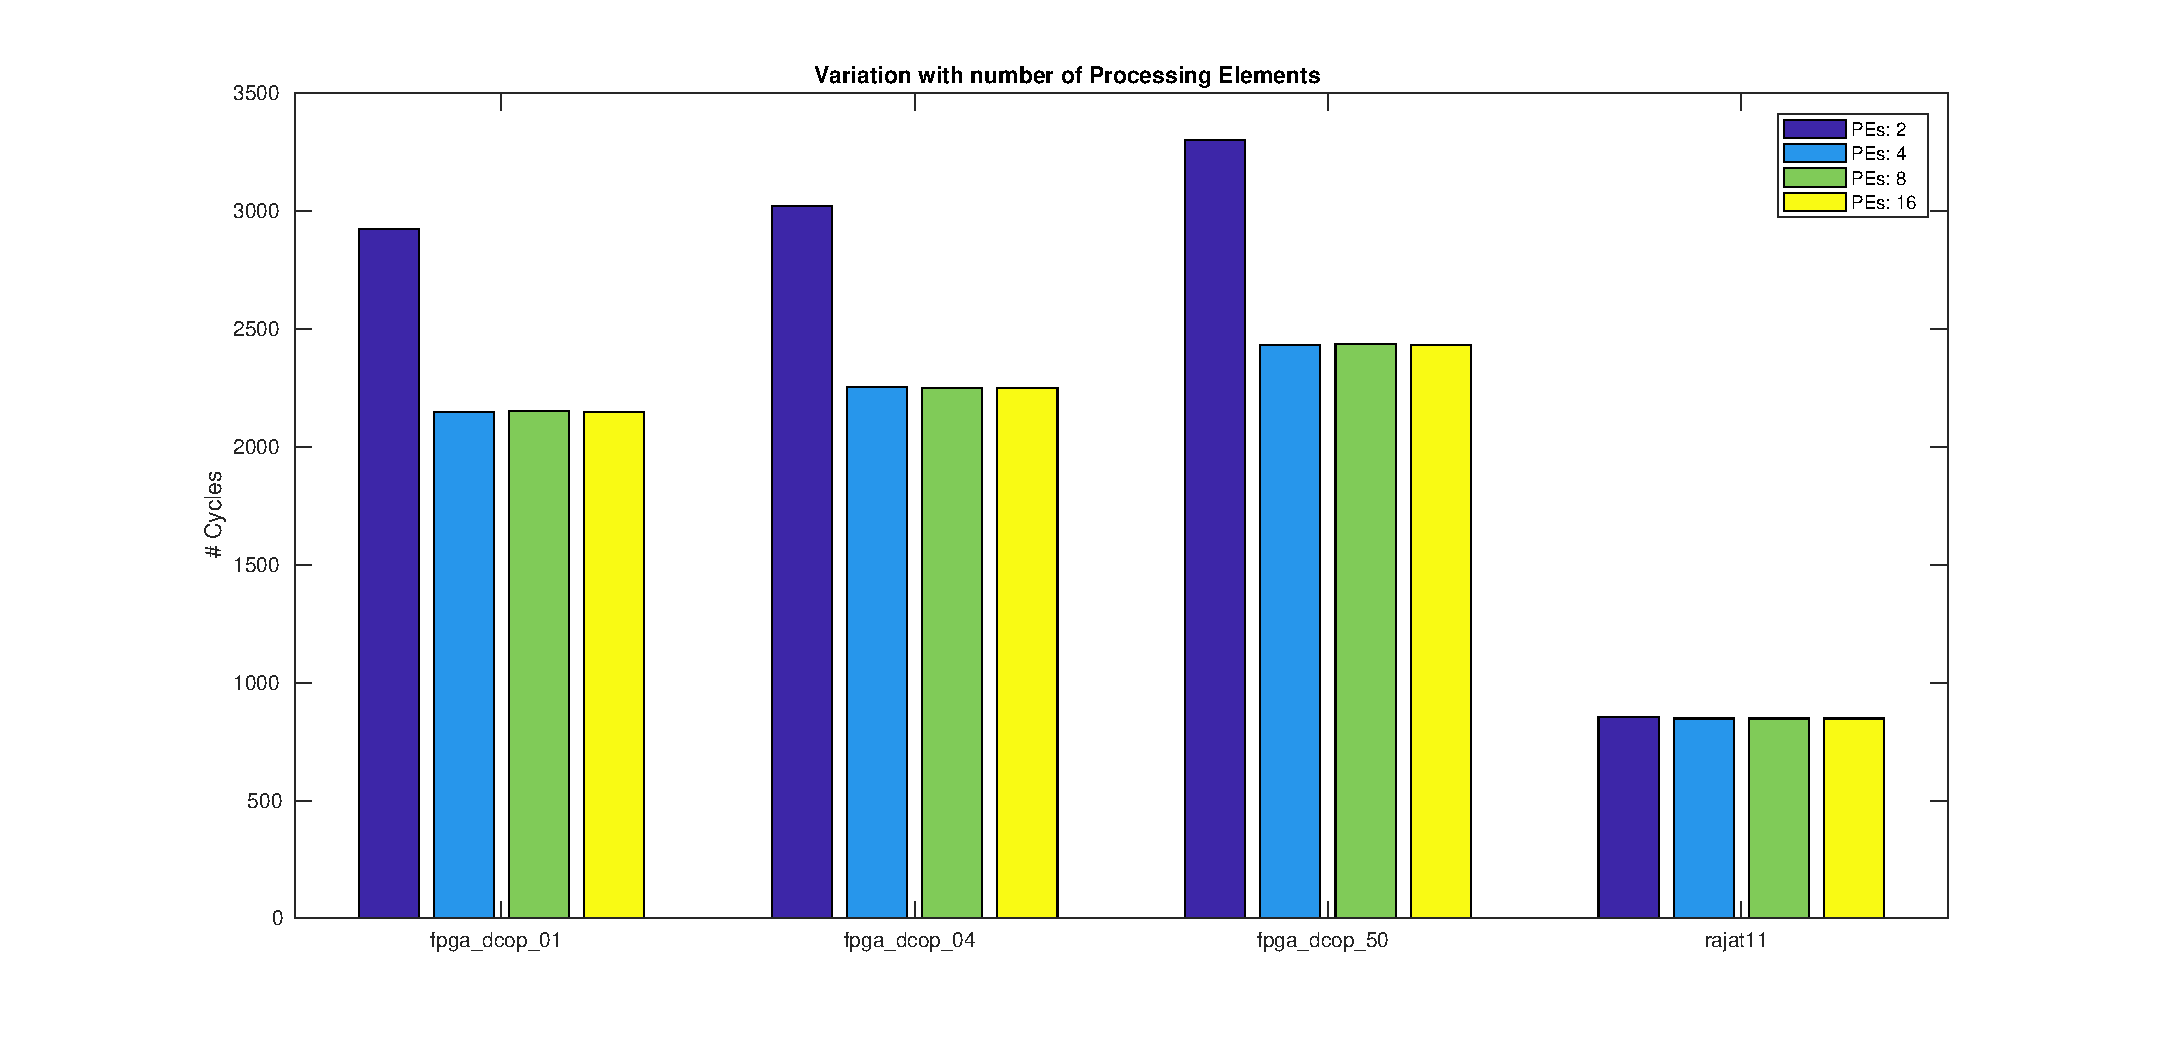
\includegraphics[width = \textwidth]{./Results/peVar.eps}
    \caption{Performance variation with number of Processing Elements}
    \label{fig:res:peVar:plot}
\end{figure}







\subsection{Variation with Number of BRAMs}

As the number of BRAMs increases not only the number of 
available read ports increases but also the data gets distributed over larger 
memory scape. Hence the demand over each port also reduces causing almost logarithmic
improvement in the performance. But this kind of improvement may not be scalable
because of huge amount of resources required to increase number of BRAMs.

\begin{table}[H]
    \centering
    \caption{Hardware configuration for testing variation with number of BRAMs}
    \label{tab:res:bramVar:hwConfig}
    \begin{tabular}{L{6cm} L{1.5cm}}
        \toprule
        Parameter & Value \\
        \midrule
        Number of PEs           & 16  \\
        Number of BRAMs         & Variable         \\
        Number of Ports/ BRAM   & 4         \\
        Read Latency of BRAM    & 2          \\
        Latency of MAC Unit     & 20          \\
        Latency of Divider Unit & 31          \\
        \bottomrule
    \end{tabular}
\end{table}

\begin{table}[H]
    \centering
    \caption{Performance variation with the number of BRAMs}
    \label{tab:res:bramVar:data}
    \begin{tabular}{l l l l l l} 
        \toprule
        Matrix Name & Order  & NNZ & 4 BRAMs& 8 BRAMs & 16 BRAMs \\
        \midrule
        $fpga\_dcop\_01$ & 1813 & 5892 &         2572    &    2336     &   2150   \\
        $fpga\_dcop\_04$ & 1220 & 5884 &         2639    &    2411     &   2252   \\
        $fpga\_dcop\_50$ & 1220 & 5892 &         2884    &    2616     &   2431   \\
        $rajat11$      & 135  &  665   &          846    &     849     &    848    \\
        \bottomrule
    \end{tabular}
\end{table}

\begin{figure}[H]
    \centering
    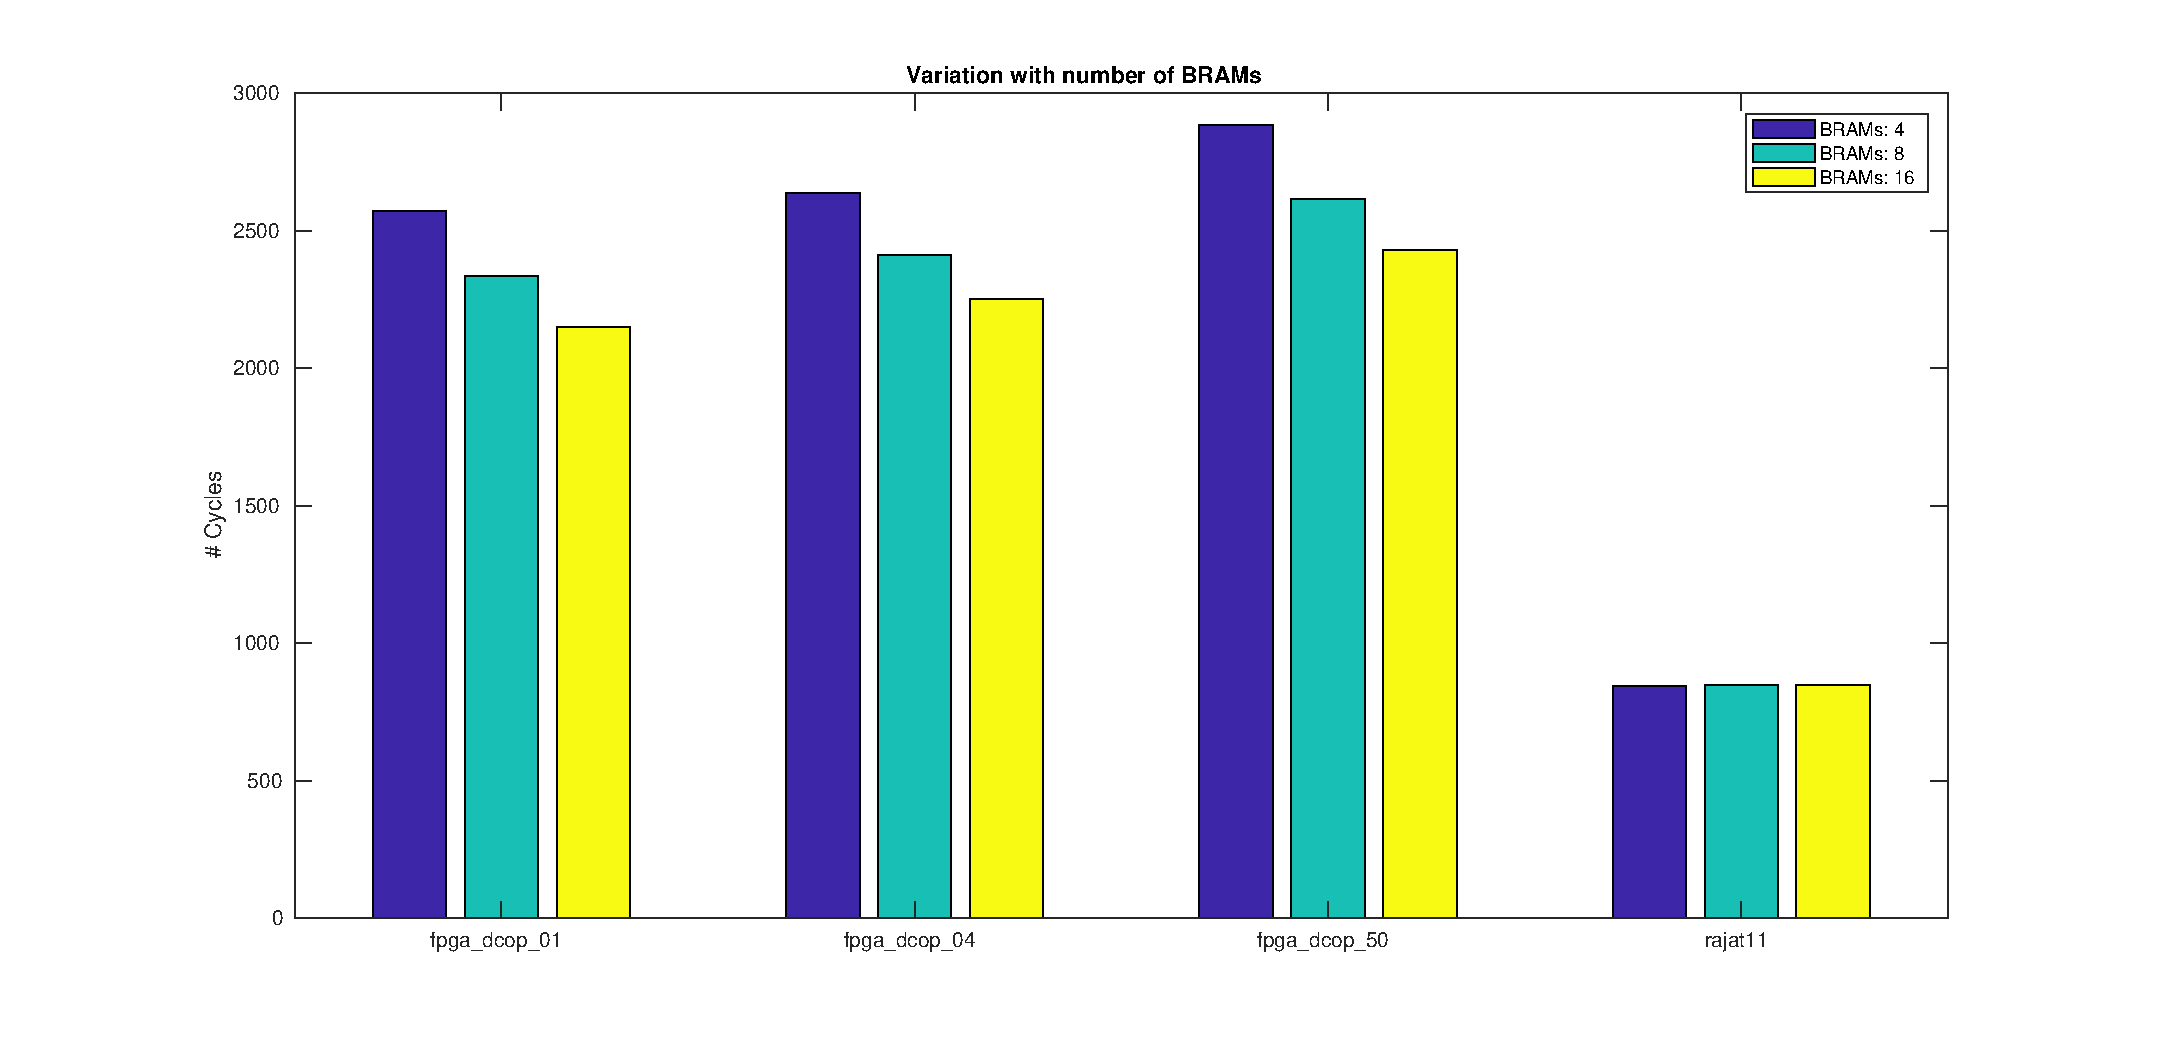
\includegraphics[width = \textwidth]{./Results/bramVar.eps}
    \caption{Performance variation with number of  BRAMs}
    \label{fig:res:bramVar:plot}
\end{figure}










\subsection{Variation with Number of Ports per BRAMs}

More number of ports per BRAM facilitates more number of simultaneous operations
on a single BRAM. The results in the figure \ref{fig:res:portVar:plot} confirm
the assertion. Though the performance improves with number of ports, returns per
port is diminishing. Also more number of ports will required more and larger multiplexers.
This multiplexers will cause routing congestion around this ports severely increasing
the synthesis time.

\begin{table}[H]
    \centering
    \caption{Hardware configuration for testing variation with number of ports per BRAMs}
    \label{tab:res:portVar:hwConfig}
    \begin{tabular}{L{6cm} L{1.5cm}}
        \toprule
        Parameter & Value \\
        \midrule
        Number of PEs           & 16  \\
        Number of BRAMs         & 16         \\
        Number of Ports/ BRAM   & Variable         \\
        Read Latency of BRAM    & 2          \\
        Latency of MAC Unit     & 20          \\
        Latency of Divider Unit & 31          \\
        \bottomrule
    \end{tabular}
\end{table}

\begin{table}[H]
    \centering
    \caption{Performance variation with the number of ports per BRAMs}
    \label{tab:res:portVar:data}
    \begin{tabular}{l l l l l l l} 
        \toprule
        Matrix Name & Order  & NNZ & 3 Ports & 4 Ports & 5 Ports & 6 Portss \\
        \midrule
        $fpga\_dcop\_01$ & 1813 & 5892 &         2551   &     2150     &   2020    &    1920   \\
        $fpga\_dcop\_04$ & 1220 & 5884 &         2651   &     2252     &   2179    &    2112   \\
        $fpga\_dcop\_50$ & 1220 & 5892 &         2871   &     2431     &   2358    &    2281   \\
        $rajat11$      & 135  &  665   &          845   &      848     &    843    &     843    \\
        \bottomrule
    \end{tabular}
\end{table}

\begin{figure}[H]
    \centering
    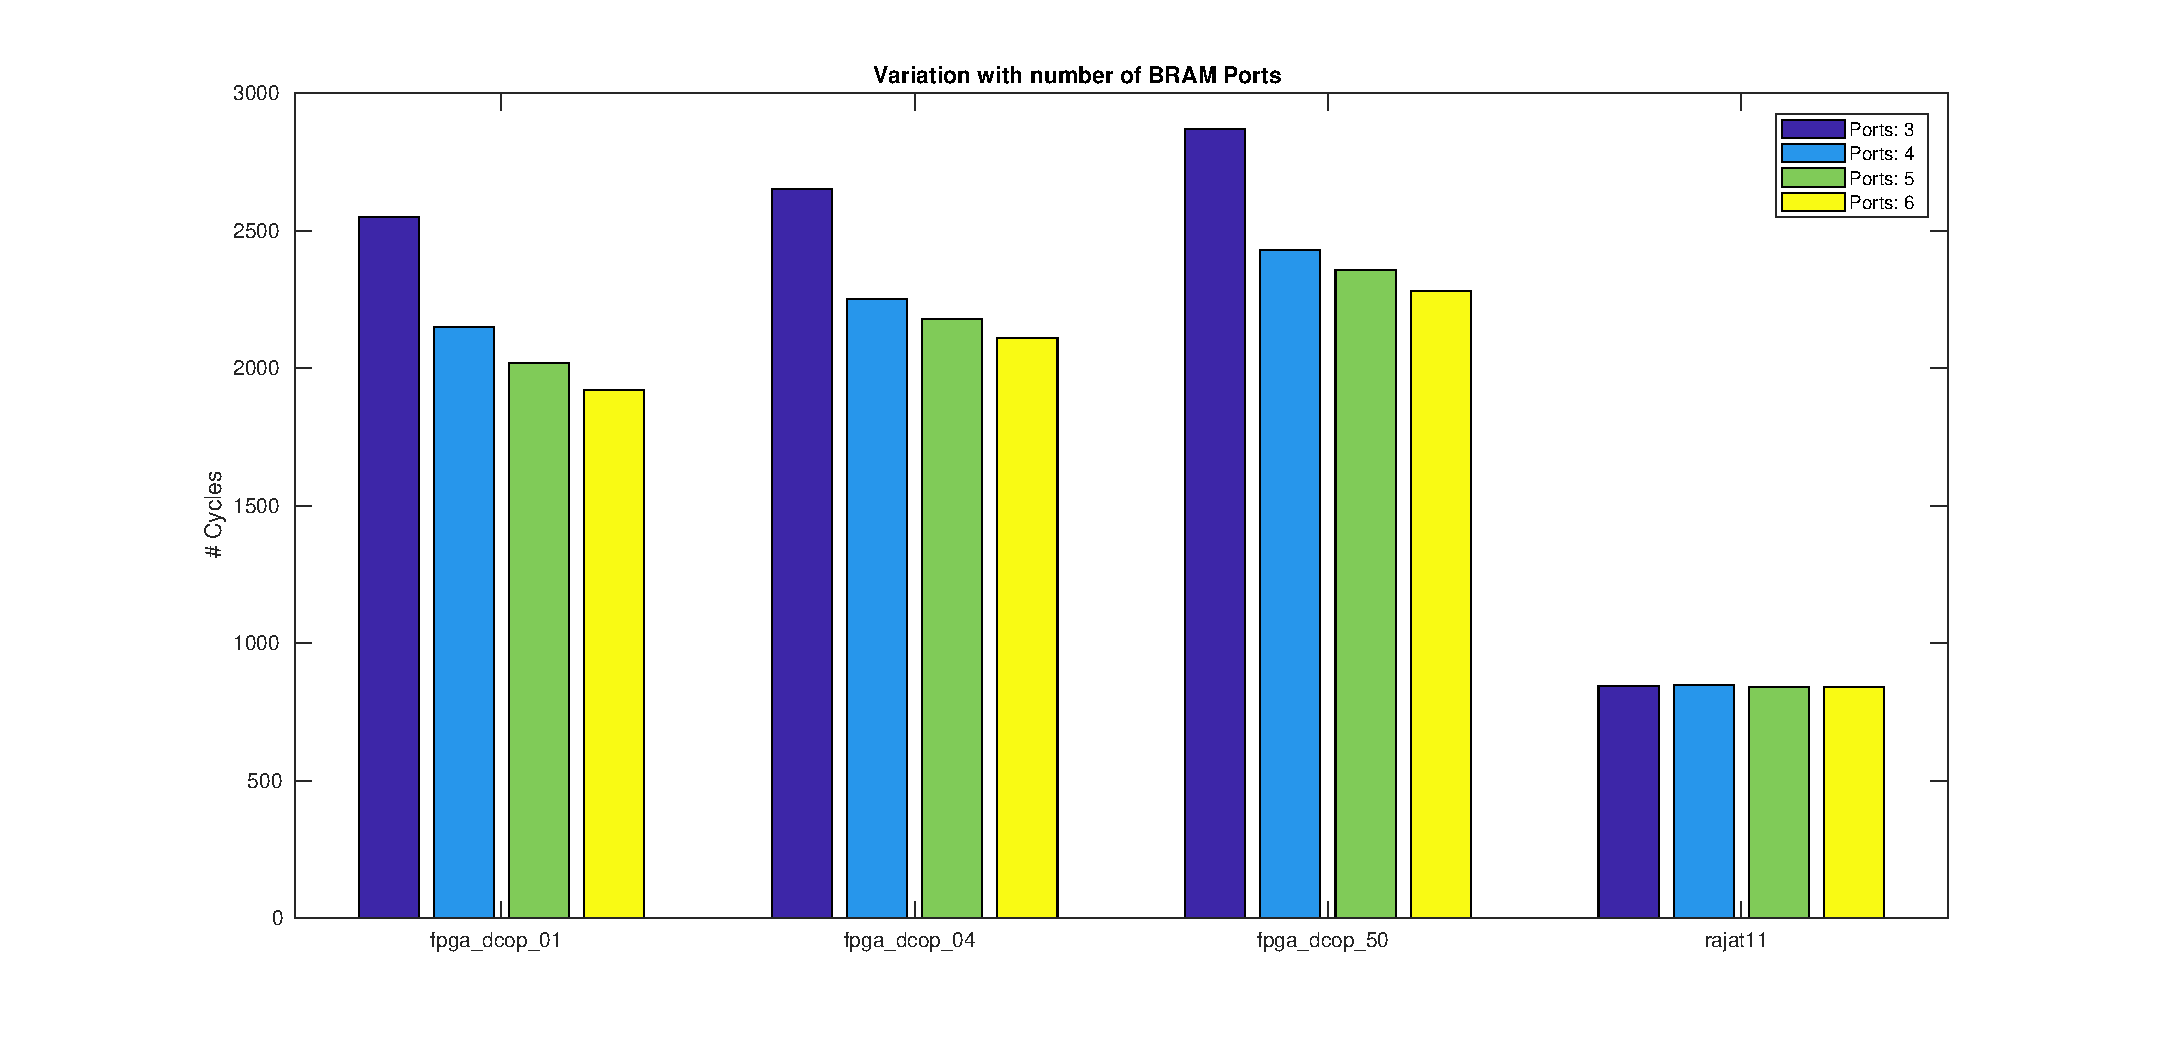
\includegraphics[width = \textwidth]{./Results/portVar.eps}
    \caption{Performance variation with number of Ports per BRAM}
    \label{fig:res:portVar:plot}
\end{figure}







\subsection{Variation with the Read Latency of BRAMs}

As expected the read latency should not affect the performance much because 
the scheduler tries to parallelize the tasks keeping the latency in check and the 
data dependence is unaffected by he latency hence the relative schedule of the nodes
remain the same.

\begin{table}[H]
    \centering
    \caption{Hardware configuration for testing variation with latency of BRAMs}
    \label{tab:res:barmLatVar:hwConfig}
    \begin{tabular}{L{6cm} L{1.5cm}}
        \toprule
        Parameter & Value \\
        \midrule
        Number of PEs           & 16  \\
        Number of BRAMs         & 16         \\
        Number of Ports/ BRAM   & 4         \\
        Read Latency of BRAM    & Variable          \\
        Latency of MAC Unit     & 20          \\
        Latency of Divider Unit & 31          \\
        \bottomrule
    \end{tabular}
\end{table}

\begin{table}[H]
    \centering
    \caption{Performance variation with the read latency of BRAMs}
    \label{tab:res:bramLatVar:data}
    \begin{tabular}{l l l l l l l} 
        \toprule
        Matrix Name & Order  & NNZ & Latency 2 & Latency 4 & Latency 6  \\
        \midrule
        $fpga\_dcop\_01$ & 1813 & 5892 &         2150  &      2143   &     2147    \\
        $fpga\_dcop\_04$ & 1220 & 5884 &         2252  &      2252   &     2263    \\
        $fpga\_dcop\_50$ & 1220 & 5892 &         2431  &      2436   &     2449    \\
        $rajat11$      & 135  &  665   &          848  &       867   &      868     \\
        \bottomrule
    \end{tabular}
\end{table}

\begin{figure}[H]
    \centering
    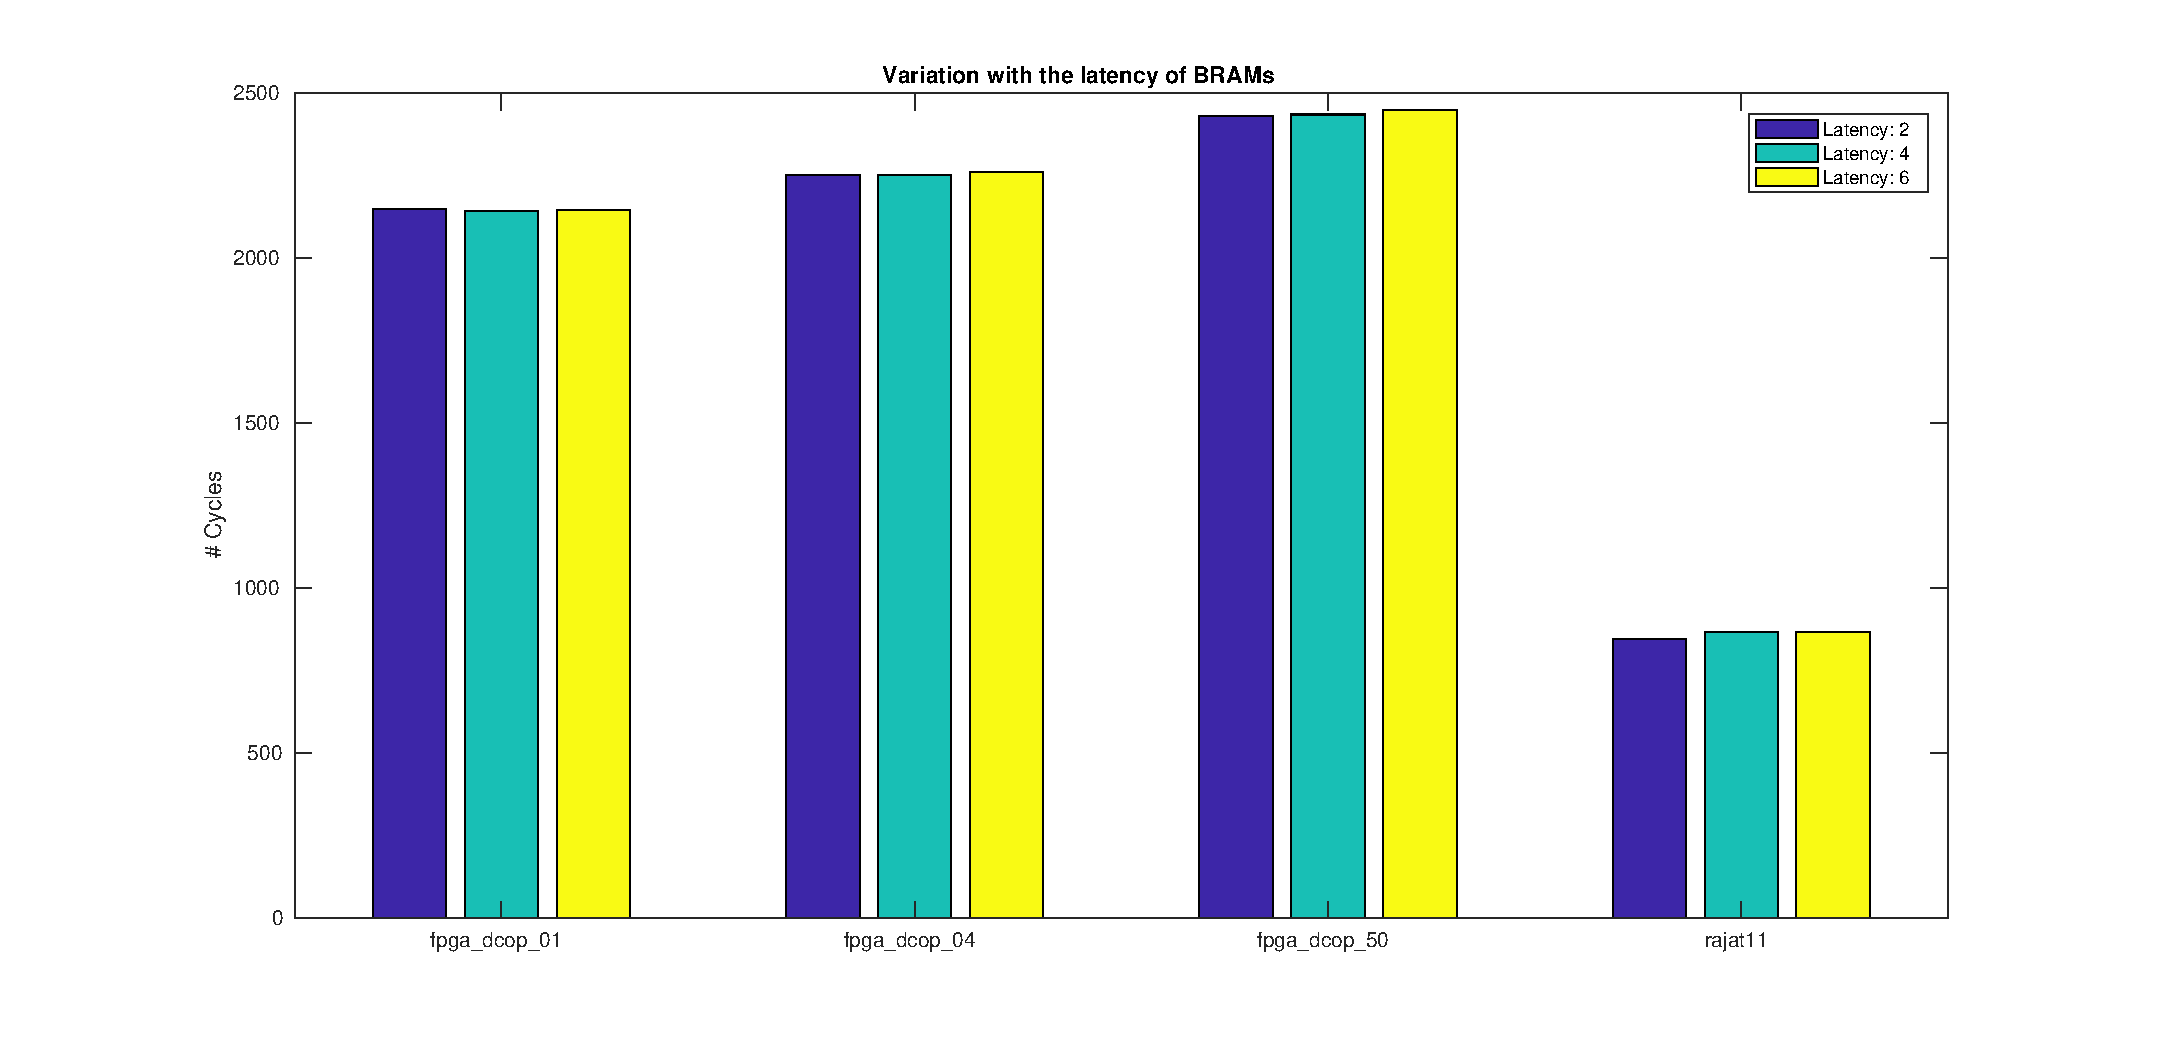
\includegraphics[width = \textwidth]{./Results/bramLatVar.eps}
    \caption{Performance variation with the read latency of BRAMs}
    \label{fig:res:bramLatVar:plot}
\end{figure}



\subsection{Variation with Ready Latency of Processing Elements}
The latency of the PEs should not affect the performance greatly because the 
latency does not affect the data dependency. The scheduler just have to delay every operation 
in the connected portion of the graph. As we have discussed in the chapter \ref{chapter:parLU}, 
the scheduler can find coarse-grain parallelism between independent sets of column and can
schedule them in the additional cycles required due to larger delays of the PEs.

Following figures confirms the above stated argument.
\begin{figure}[H]
    \centering
    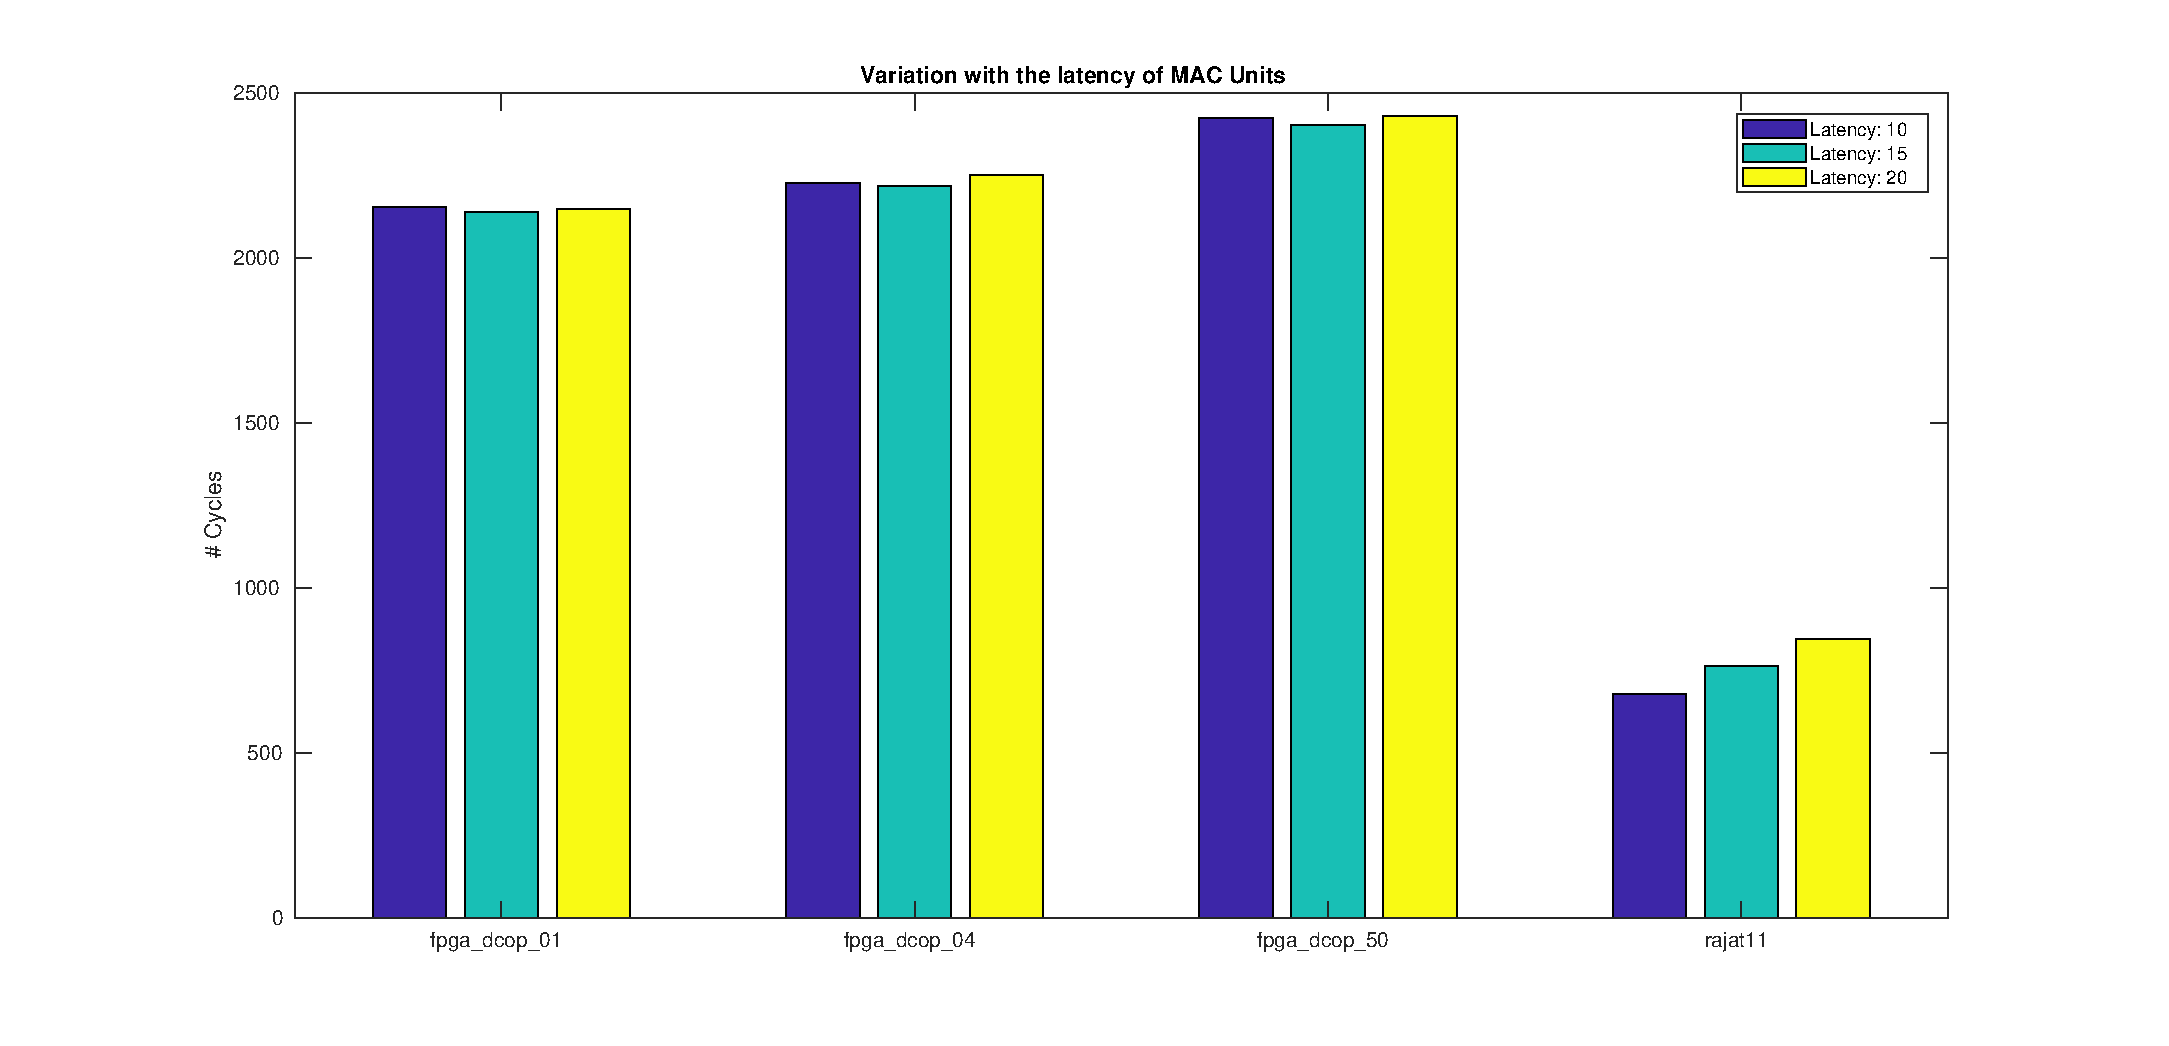
\includegraphics[width = 0.8\textwidth]{./Results/macLatVar.eps}
    \caption{Performance variation with the latency of MAC units}
    \label{fig:res:macLatVar:plot}
\end{figure}

\begin{figure}[H]
    \centering
    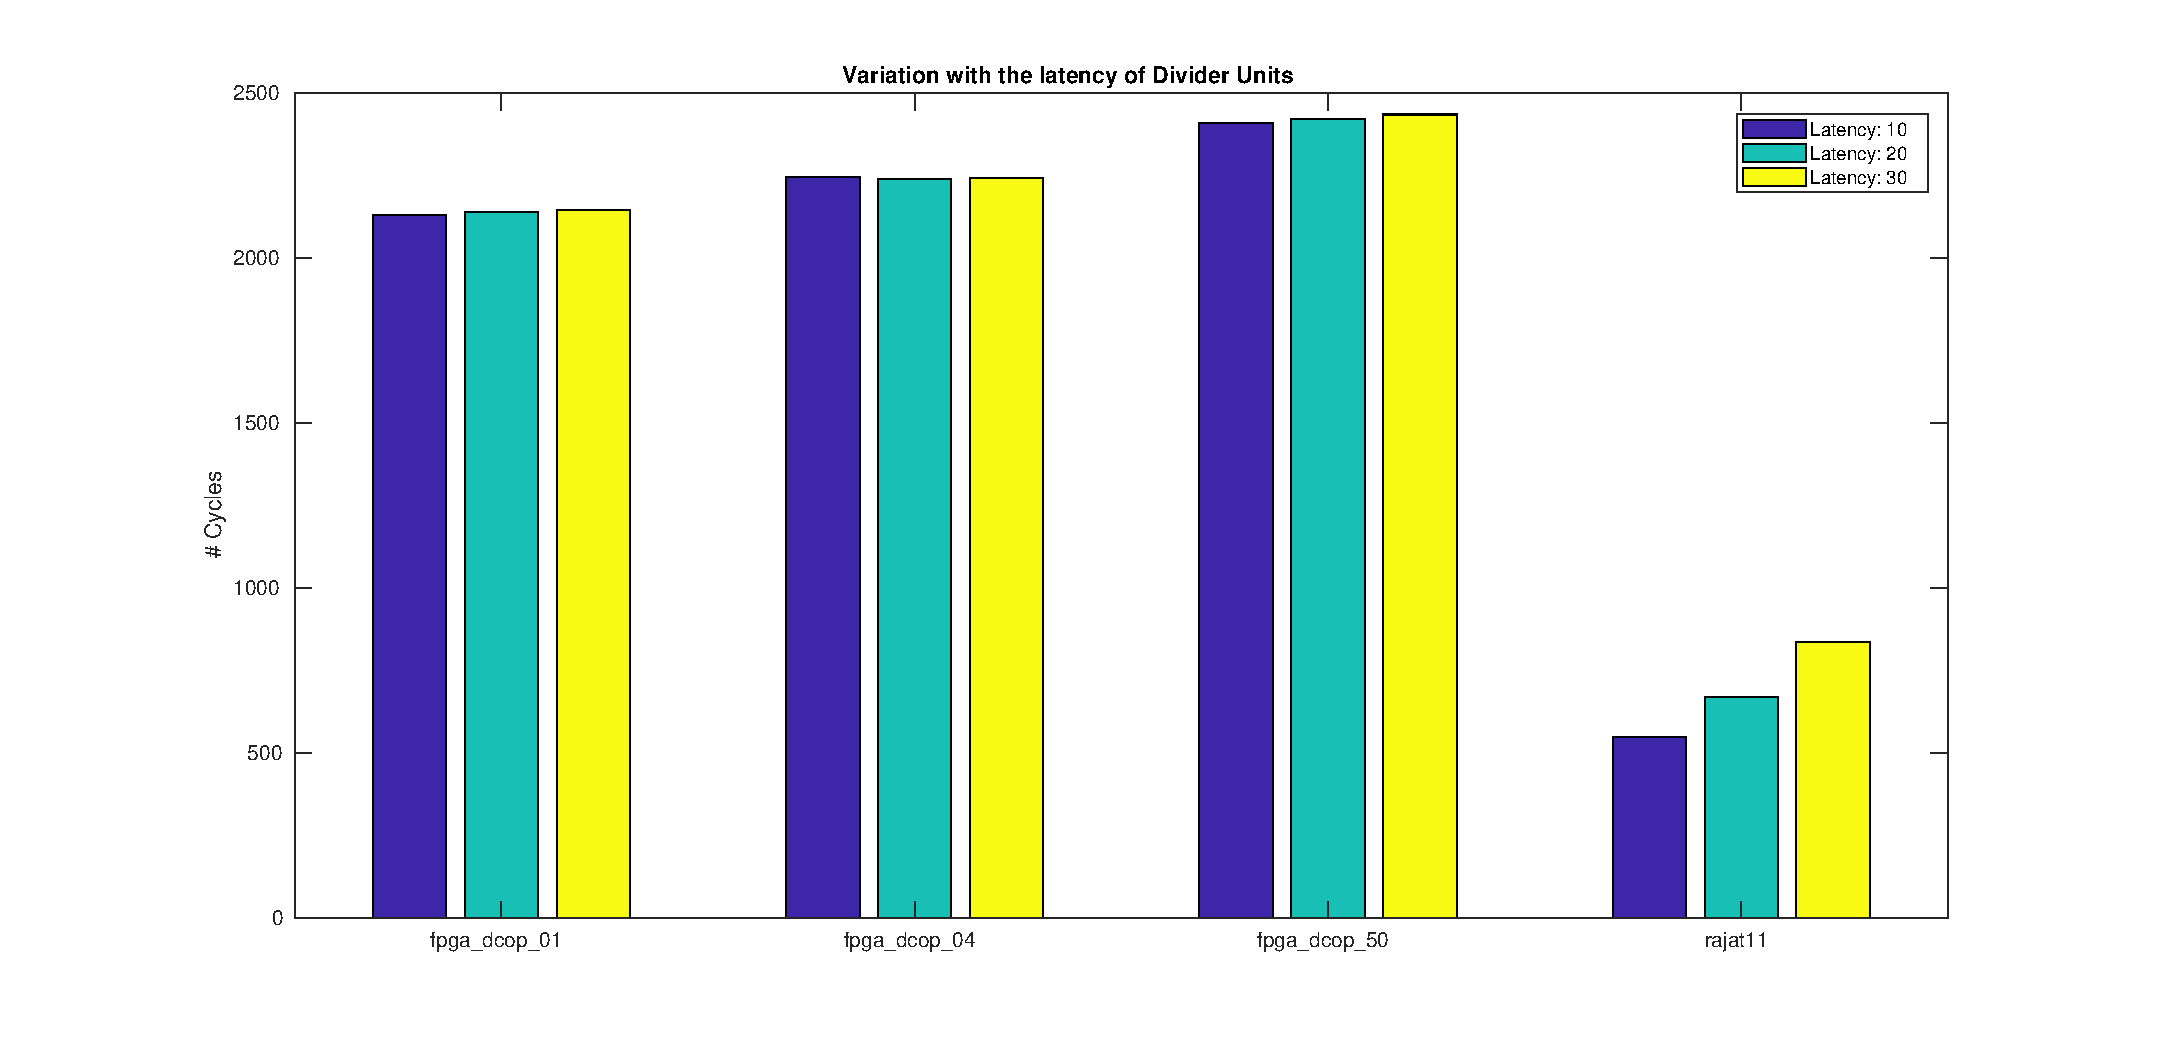
\includegraphics[width = 0.8\textwidth]{./Results/divLatVar.eps}
    \caption{Performance variation with the latency of divider units}
    \label{fig:res:divLatVar:plot}
\end{figure}

% MAC Latency Var
% 2157        2140        2150
% 2228        2220        2252
% 2424        2405        2431
%  680         765         848


% Div Latency Var

%         2132        2142        2148
%         2246        2242        2244
%         2410        2422        2436
%          550         671         837




\subsection{Comparison with Literature}
Kapre \cite{Kapre} has used intermediate matrices from the SPICE simulation to 
benchmark his system. These matrices are not available hence can not be compared with.
Nechma \cite{Nechma} has SuiteSparse matrices hence we are going to compare the performance of 
scheduling with Nechma's results. To maintain the fairness, we are going to use 
a hardware configuration similar to the \cite{Nechma}. The hardware configuration is 
mentioned in the following table:


\begin{table}[H]
    \centering
    \caption{Hardware configuration for testing variation with latency of BRAMs}
    \label{tab:res:barmLatVar:hwConfig}
    \begin{tabular}{L{6cm} L{1.5cm}}
        \toprule
        Parameter & Value \\
        \midrule
        Number of PEs           & 16  \\
        Number of BRAMs         & 16         \\
        Number of Ports/ BRAM   & 4         \\
        Read Latency of BRAM    & 2          \\
        Latency of MAC Unit     & 8          \\
        Latency of Divider Unit & 29          \\
        \bottomrule
    \end{tabular}
\end{table}


\begin{table}[H]
    \centering
    \caption{Performance variation with the read latency of BRAMs}
    \label{tab:res:bramLatVar:data}
    \begin{tabular}{l l l l l l} 
        \toprule
        Matrix Name & Order  & NNZ & Our Method & Nechma's Method \\
        \midrule
        $fpga\_dcop\_01$ & 1813 & 5892 &  2271    &  7055   \\
        $fpga\_dcop\_50$ & 1220 & 5892 &   2340   &   3047  \\
        $rajat11$      & 135  &  665   &    596   &    249    \\
        \bottomrule
    \end{tabular}
\end{table}

\begin{figure}[H]
    \centering
    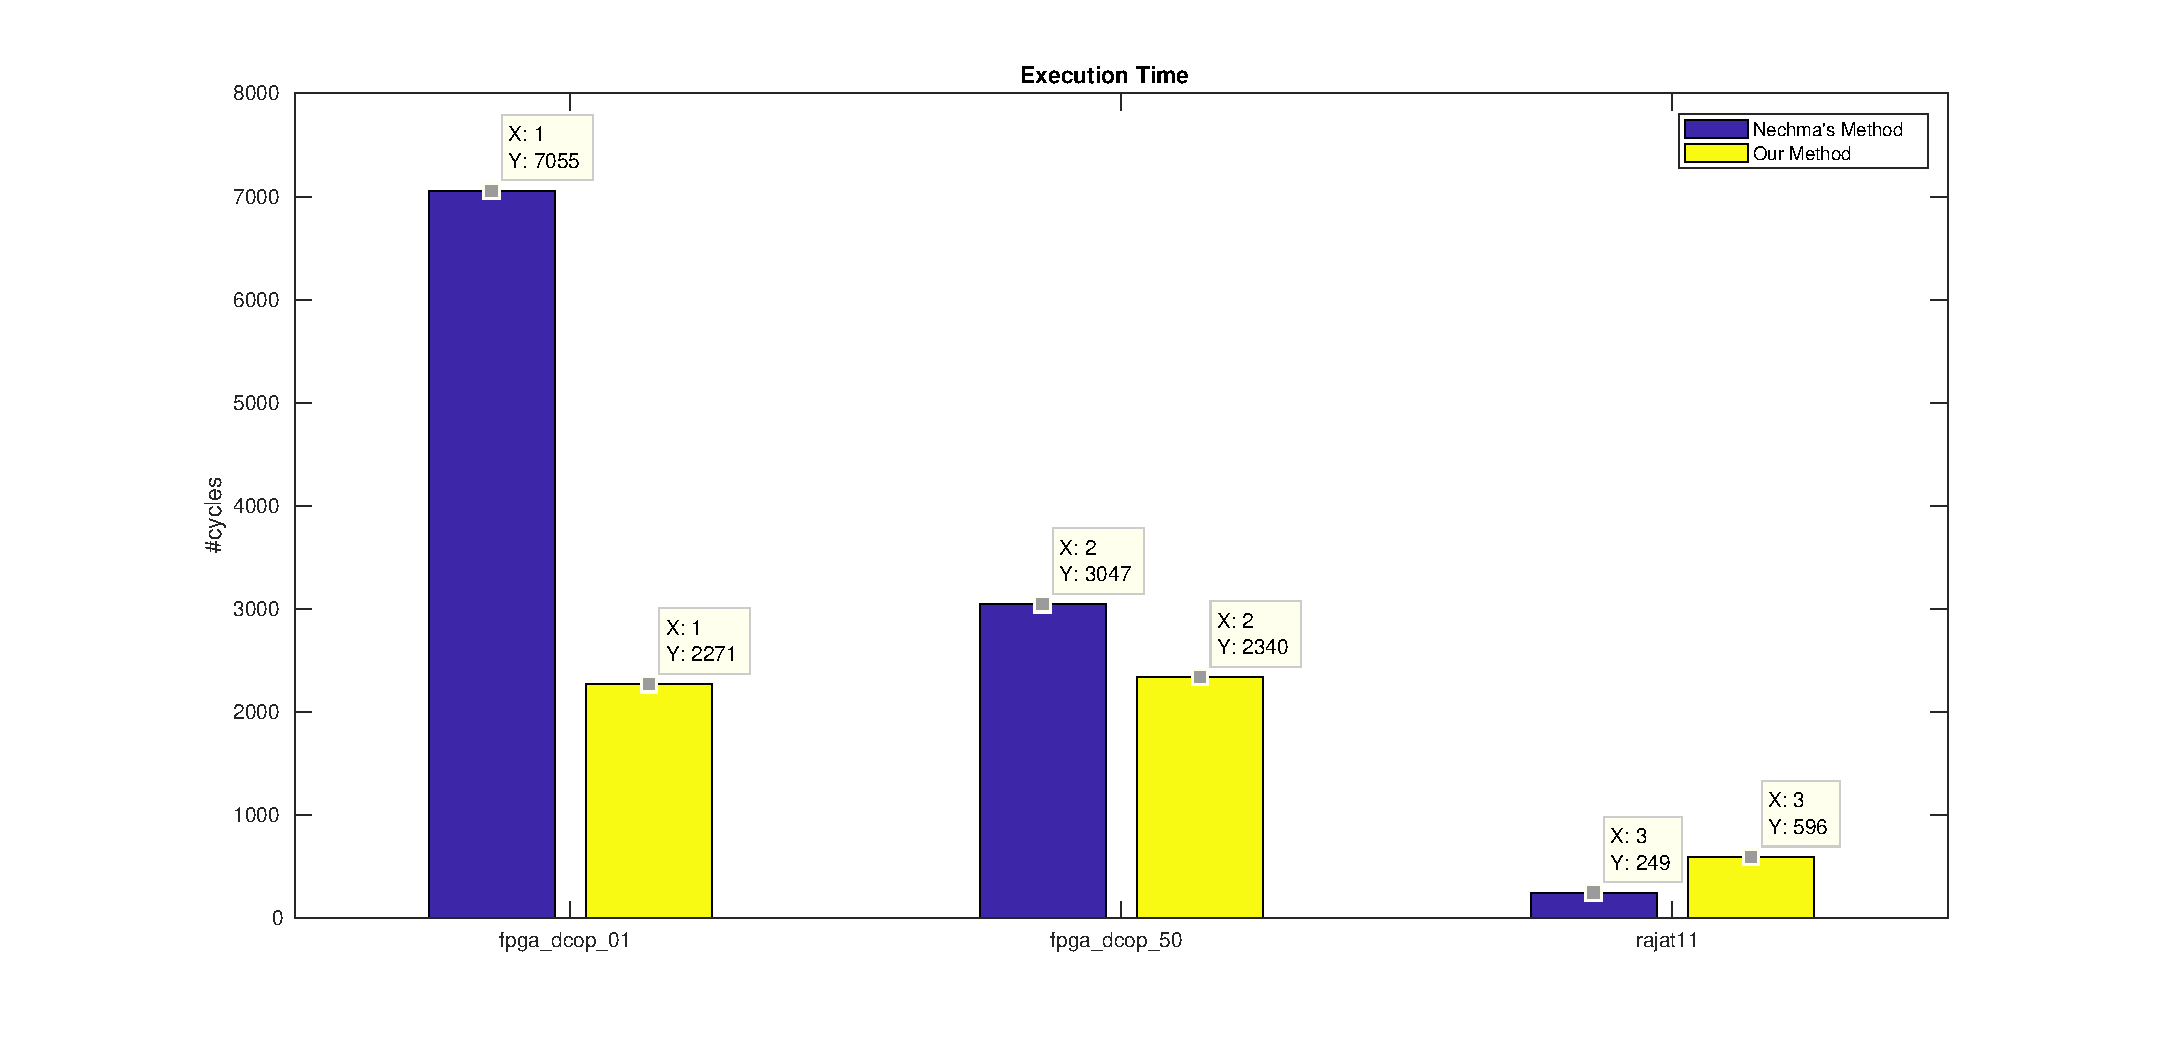
\includegraphics[width = \textwidth]{./Results/cmp.eps}
    \caption{Performance comparison between Nechma's \cite{Nechma} results and our method}
    \label{fig:res:cmp:plot}
\end{figure}

As evident form the figure \ref{fig:res:cmp:plot}, our method can extract more parallelism
and utilize the hardware more efficiently. The execution speedup is obviously
at the cost of preprocessing time.

\pagebreak

\section{Hardware Testing}
The hardware is being tested on using the Diligent's Zybo board wic has
the Zynq 7010 SoC. This is a fairly small FPGA, hence the synthesized hardware 
can not be too large. The hardware being tested has the configuration as mentioned in the table 
\ref{tab:res:hwTesting:hwConfig}. 

\begin{figure}[H]
    \centering
    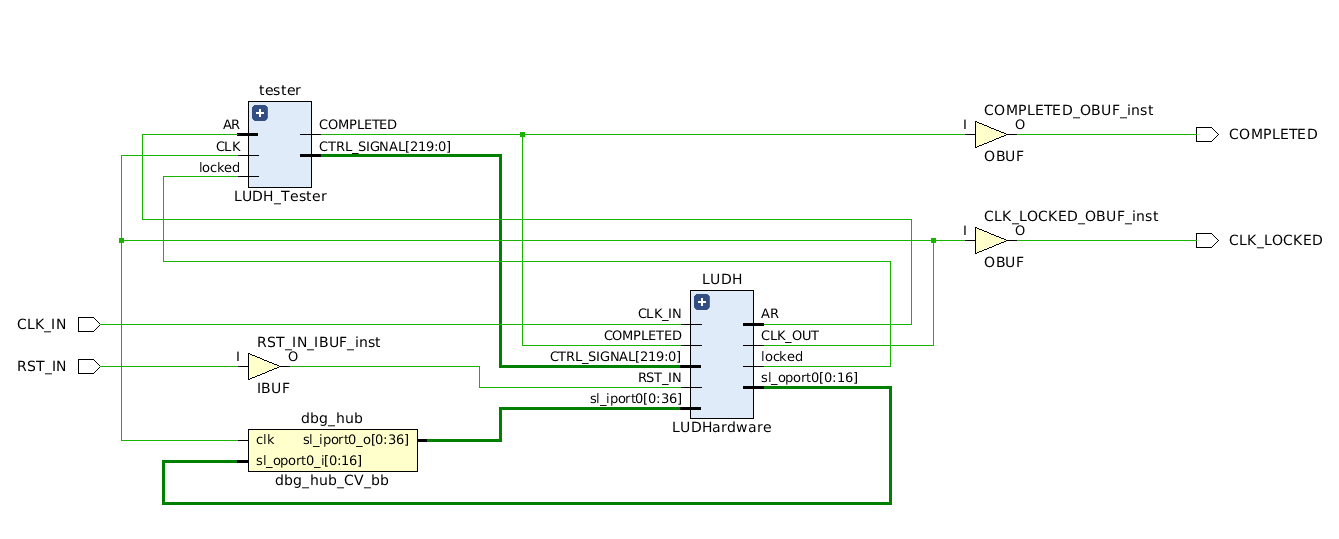
\includegraphics[width = 0.9\linewidth]{./Results/synHardware.png}
    \caption{Schematic of the synthesized hardware}
    \label{fig:res:synHwdd}
\end{figure}

For testing purposes the hardware is wrapped inside a synthesizable test bench 
which includes instruction and input matrix storage. This testbench emulates 
the behavior of master and main memory. 

\begin{table}[H]
    \centering
    \caption{Hardware configuration testing on FPGA}
    \label{tab:res:hwTesting:hwConfig}
    \begin{tabular}{L{6cm} L{1.5cm}}
        \toprule
        Parameter & Value \\
        \midrule
        Number of PEs           & 4  \\
        Number of BRAMs         & 4         \\
        Number of Ports/ BRAM   & 4         \\
        Read Latency of BRAM    & 2          \\
        Latency of MAC Unit     & 20          \\
        Latency of Divider Unit & 31          \\
        \bottomrule
    \end{tabular}
\end{table}


The operating frequency of the system is 
set at 100 MHz and it is generated using the PLL as mentioned in the hardware section.
The hdl generation tool also generate additional board files to incorporate
Hardware Integrated Logic Analyzer to debug and capture the on-chip waveforms.

At this stage all the components of the hardware except Quad Port BRAMs are working 
properly. The figure \ref{fig:res:synHwdd} shows the schematic of synthesized hardware.


\begin{figure}
    \centering
    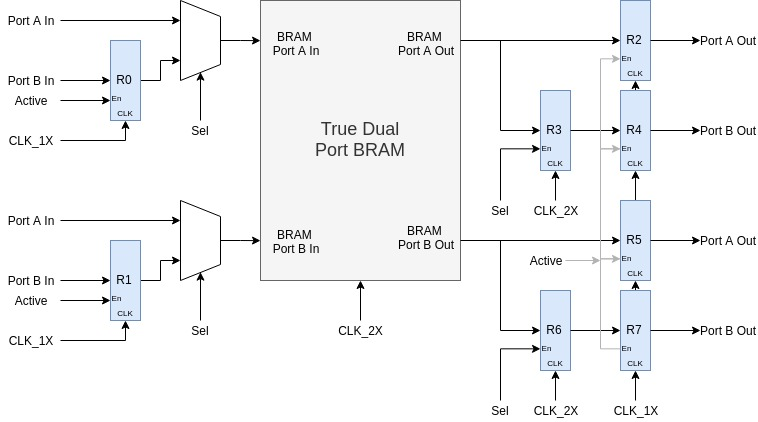
\includegraphics[width = 0.9\linewidth]{./Results/quadPortBRAM.jpg}
    \caption{BRAM unit with 4 time multiplexed ports}
    \label{fig:res:bram}
\end{figure}

\begin{figure}
    \centering
    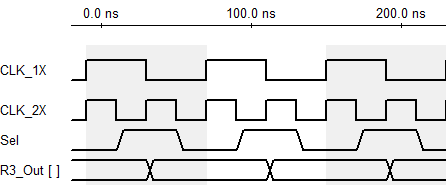
\includegraphics[width = 0.9\textwidth]{./Results/bramWaveProblem.png}
    \caption{Location of false hold violation}
    \label{fig:res:wave}
\end{figure}

\textbf{The Problem}\\
As we have discussed in the previous chapters the time multiplexed ports requires 
two separate clock sources with the ratio of operating frequencies 2:1. The figure 
\ref{fig:res:bram} shows the structure of the BRAM. If we look at the path between
registers $R3$ and $R4$, the path is sensitized by the faster clock and it 
acts as the input for the path in slower clock domain. As we have seen from the 
waveforms before, there is nothing wrong with this because the output of the 
register $R3$ is not going to change when $R4$ samples it because the $Sel$ signal
is low at the rising edge of the slower clock. But the timing analyzer flags it for the 
hold violation as it assumes that the output of $R3$ is going to change at every clock
cycle. 







\begin{figure}
    \centering
    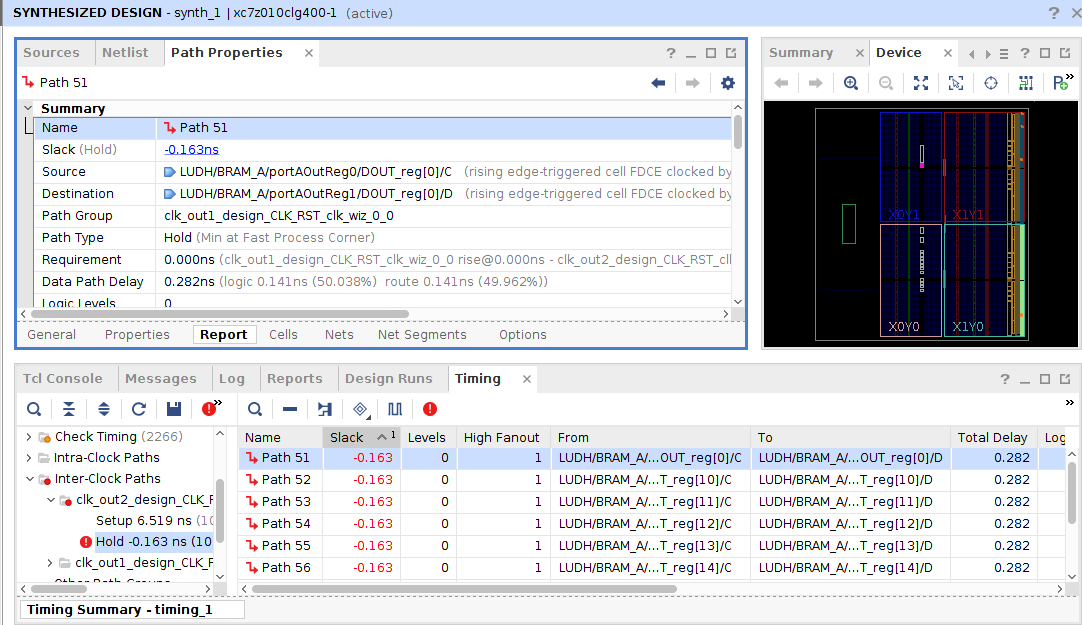
\includegraphics[width = \linewidth]{./Results/timingRepor.png}
    \caption{Hold violation reported by the synthesis tool}
    \label{fig:res:bram}
\end{figure}



